\chapter{Development Methodology}

In this project it was chosen to follow an iterative development process. This was chosen because the success criteria for this project is not well defined~\cite{dahlbom1993computers}. The goal of picking which track to play next is a largely subjective decision.

This project being very experimental meant that following a linear approach could require a large amount of research, which has not previously been done, for making descriptive analysis and design documents, before being able to test our solution. Problems, which arise later in the process, would then not be handled in an efficient way.

One of the problems with the incremental model compared to the linear waterfall model is that the project can lack structure, since setting milestones with clear goals can be difficult.

\section{Iterative Design Process}
\label{IterativeDesignProcess}
In the iterative process, the design and implementation is done one
step at a time. The development is done in iterations, with a new
milestone for each iteration. An overview of the process can be seen
in \cref{fig:developmentprocess}. These milestones consist of some
features which will be analysed, designed, implemented and evaluated,
documenting every step in the process. Users will be interviewed in an
effort to find new possible problems or requirements, to be taken up
for consideration in the following iterations. The following steps
will be followed through each iteration:

\begin{enumerate}
  \item Gathering data from users and previous iterations
  \item A brief analysis of these data, for declaring new requirements
  \item A comprehensive design phase, researching and choosing concepts in solving these requirements
  \item An implementation period, implementing the chosen design
  \item Evaluation, consisting mainly of black- and white box testing
\end{enumerate}

\begin{figure}[hbtp]
  \centering
  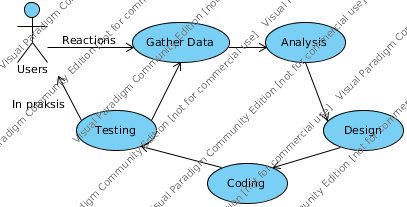
\includegraphics[width=1\linewidth]{Developmentprocess}
  \caption{Overview of the iterative development methodology.}\label{fig:developmentprocess}
\end{figure}

\subsection{Iterations}

Throughout the project, the deadlines of the individual iterations were planned according to the project group's semester courses. The first iteration was longer, in order to get the initial prototype working.

\subsubsection{1\textsuperscript{st} Iteration}

The project group set out with following milestones for the first iteration:

Milestones
\begin{itemize}
        \item Interview bars and pubs about requirements of a music system for their venue
        \item Initial data structure
        \item Be able to vote on a track
        \item Communicate a request for a track from one device to another and play it
\end{itemize}

The project group started out with a requirement of being able to count votes on specific tracks, but went a little behind schedule, due to unforeseen details about libspotify, so it was simplified to just communicating with the server.

In hindsight, this was too ambitious. The iteration did not account
for the time to learn the Spotify platform. In the following iterations, planning for learning tools should be accounted for. Not every decision in the design phase was documented in the report. In addition, no significant testing was made.

\subsubsection{2\textsuperscript{nd} Iteration}

After the experience made in previous iterations, about being too
ambitious in meeting all milestones at deadline, another approach is
introduced, by classifying each milestone under what \emph{Must} and
what \emph{Should} be done in this iteration. An emphasise will be put on documentation and testing on milestones of 2nd iteration:

Must
\begin{itemize}
        \item Interview everyday users about requirements for music systems
        \item Do a section on concepts in the system
\end{itemize}

Should
\begin{itemize}
        \item Document previously taken decisions
        \item Describe the architecture
        \item Do a comprehensive testing section
        \item Make a democratic voting implementation on the backend
\end{itemize}

\subsubsection{3\textsuperscript{rd} Iteration}

The way of making goals for the iterations changed yet again, to making specific goals for each step in the development cycle. This means we could conclude on each step of the cycle, which showed to be beneficial, in that we could track the progression of each concept, included in the project through the development cycle from \enquote{Data Collection} to \enquote{Testing}.

Gather Data
\begin{itemize}
  \item Interview and showcase demo for collaboration partner \enquote{Fabrikken}
\end{itemize}

Analysis
\begin{itemize}
  \item Document interview with collaboration partner
  \item Extract requirements
  \item Revisit classes to account for restrictions
\end{itemize}

Design
\begin{itemize}
  \item Restriction design
  \item Revisit Architecture
\end{itemize}

Implementation
\begin{itemize}
  \item Implement restriction design
  \item Document patterns used for this
\end{itemize}

Testing
\begin{itemize}
  \item Test that restrictions works as intended by unit testing
  \item Test restrictions in context of users
\end{itemize}

\subsubsection{4\textsuperscript{th} Iteration}

This iteration reused the method of making goals from the
3\textsuperscript{rd} iteration.  The same process as previous
iterations were followed. A presentation interface was designed and implemented.
